\documentclass[12pt]{article}
\usepackage{graphicx}
\usepackage{geometry}
\usepackage{float}
\usepackage{amsmath}
\usepackage[italian]{babel}
\usepackage{listings,xcolor}
\definecolor{javared}{rgb}{0.6,0,0} % for strings
\definecolor{javagreen}{rgb}{0.25,0.5,0.35} % comments
\definecolor{javapurple}{rgb}{0.5,0,0.35} % keywords
\definecolor{javadocblue}{rgb}{0.25,0.35,0.75} % javadoc

\lstset{
  tabsize = 4, %% set tab space width
  showstringspaces = false, %% prevent space marking in strings, string is defined as the text that is generally printed directly to the console
  numbers = left, %% display line numbers on the left
  keywordstyle=\color{javagreen}\bfseries,
  stringstyle=\color{javared},
  commentstyle=\color{javagreen},
  morecomment=[s][\color{javadocblue}]{/*}*{*/},
  rulecolor = \color{black}, %% set frame color to avoid being affected by text color
  basicstyle = \small \ttfamily , %% set listing font and size
  breaklines = true, %% enable line breaking
  numberstyle = \tiny,
}



\begin{document}
\begin{titlepage}
   \begin{center}
       \vspace*{1cm}
	   \begin{Huge}
       \textbf{Valutazione performance InsertionSort e MergeSort}
	   \end{Huge}
       \vspace{1.5cm}
       \\
       \begin{Large}
        Relazione esercizio 1
            
       \vspace{1.5cm}

       Laboratorio di Algoritmi e Strutture Dati
	   \vspace{3cm}
            
       Gemma Vaggelli \\
       6348717
            
       \vfill
     
    
            
       Ingegneria Informatica\\
       Università degli studi di Firenze
       \end{Large}
       
            
   \end{center}
\end{titlepage}
\section{Introduzione}
Il problema dell'ordinamento è un problema di tipo algoritmico in cui, dato in input una sequenza di n numeri $<$ $a_1$; $a_2$; ... ; $a_n$ $>$ , genera in output una permutazione \\$<$ $a_1^{'}$; $a_2^{'}$; ... ; $a_n^{'}$ $>$ della sequenza di input tale che $<$ $a_1^{'}$ $\le$ $a_2^{'}$ $\le$ ... $\le$ $a_n^{'}$ $>$.
\\Tra i molti algoritmi di ordinamento in questo esercizio verranno trattate e valutate le performance degli algoritmi InsertionSort e MergeSort. 
\\Vogliamo valutare attraverso dei test quale dei 2 algoritmi è più efficiente; ciò verrà effettuato valutando i 2 algoritmi in base a due fattori: la velocità di esecuzione all'aumentare della lunghezza degli array e la medesima in base alla conformazione dell'array in input.

\section{Caratteristiche}
I due algoritmi presentano delle differenze sostanziali nel trattamento dell'array in input.

\subsection{Caratteristiche InsertionSort}
L'insertionSort è un algoritmo di ordinamento iterativo che si basa sull'inserimento di un elemento all'interno di un array.Il suo funzionamento è paragonabile all'operazione che si svolge quando si ordinano le carte in mano, partendo da una mano vuota e tutte le carte in tavola si pesca una carta alla volta e si inserisce nella posizione 'giusta', ovvero in maniera ordinata rispetto alle carte che si hanno in mano in quel momento. 
\subsection{Caratteristiche MergeSort}
L'algoritmo MergeSort d'altra parte è un algoritmo ricorsivo Divide et Impera e come tale, si compone di 3 fasi: 
\begin{itemize}
\item \textbf{Divide} che consiste nel dividere a metà l'array;
\item \textbf{Impera} che ordina, chiamando ricorsivamente la funzione MergeSort, i 2 sotto-array;
\item \textbf{Combina} che, all'interno della funzione Merge, prende i 2 sotto-array ordinati e forma un singolo array ordinato.
\end{itemize}
\section{Prestazioni}
\subsection{Prestazioni InsertionSort}
Dall'analisi teorica dell'algoritmo InsertionSort possiamo vedere che le prestazioni dell'algoritmo cambiano al variare della disposizione degli elementi all'interno dell'array, perciò bisogna testare le prestazioni dell'algoritmo nel caso migliore, nel caso medio e nel caso peggiore. 
\\Il caso migliore è un array di partenza già ordinato, in questo caso il tempo di esecuzione dell'algoritmo T(n) è una funzione lineare di n.
\\Il caso peggiore è un array di partenza ordinato al contrario, in questo caso T(n) è una funzione quadratica di n.
\\Nel caso medio l'algoritmo nel ciclo while fa circa la metà dei controlli rispetto a quelli che fa nel caso peggiore però T(n) rimane una funzione quadratica di n.
\subsection{Prestazioni MergeSort}
Dall'analisi teorica dell'algoritmo MergeSort si nota che le prestazioni dell'algoritmo sono pressoché le stesse qualsiasi sia la disposizione degli elementi all'interno dell'array, quindi non vi è un caso migliore o peggiore.
\\Come per gli altri algoritmi ricorsivi Divide et Impera si valuta il costo del MergeSort attraverso l'equazione di ricorrenza.
\begin{equation*}
T(n) = \begin{cases}
\Theta(1) & \text{se $n$ = 1,}\\
2T(\frac{n}{2}) + \Theta(n) & \text{se $n$ $>$ 1.}
\end{cases}
\end{equation*}
L'equazione di T(n) in forma chiusa con notazione asintotica per il MergeSort è T(n) $= \Theta(n)$


\section{Documentazione}

Il programma è formato dalle funzioni che eseguono gli algoritmi \textbf{InsertionSort} e \textbf{MergeSort}, dalla funzione \textbf{Client} che si occupa di svolgere i test e di calcolare il tempo di esecuzione di ognuno di essi e dalla funzione \textbf{BGenerator} che si occupa della creazione dei vari array su cui applicare i due algoritmi di ordinamento.
\\La funzione BGenerator prende in input la lunghezza dell'array che si vuole generare e una stringa che determina la modalità di creazione del medesimo.La funzione può generare array casuali, ordinati o ordinati al contrario.
\\All'interno della funzione Client, oltre a ciò che ho specificato sopra, viene creato un file csv per visualizzare i dati elaborati dalla funzione quali la dimensione dell'array da ordinare e il tempo impiegato (in millisecondi) da ciascun algoritmo di ordinamento.







\paragraph{Hardware}
I test sono stati eseguiti su un PC Desktop con sistema operativo Windows 10 Home a 64 bit, un processore Intel Core i5-7200U con 8Gb di RAM e Visual Studio Code come IDE.
 
\section{Prestazioni risultati sperimentali}
\subsection{Prestazioni risultati sperimentali caso Random}
\begin{center}
 \begin{tabular}{||c  c c||} 
 \hline
 Dim & Merge  & Ins \\ [0.5ex] 
\hline
0  & 0 & 0 \\
\hline
200 & 4 & 4 \\
\hline
400 & 4 & 24 \\
\hline
600 & 4 & 44 \\
\hline
800 & 8 & 68 \\
\hline
1000 & 8 & 104 \\
\hline
1200 & 16 & 224 \\
\hline
1400 & 12 & 284 \\
\hline
1600 & 20 & 392 \\
\hline
1800 & 20 & 480 \\
\hline
2000 & 28 & 540 \\
\hline
2200 & 20 & 600 \\
\hline
2400 & 24 & 640 \\
\hline
2600 & 28 & 992 \\
\hline
2800 & 28 & 936 \\
\hline
3000 & 32 & 1088 \\
\hline
3200 & 48 & 1172 \\
\hline
3400 & 32 & 1440 \\
\hline
3600 & 48 & 1644 \\
\hline
3800 & 36 & 1972 \\
\hline
4000 & 48 & 2136 \\
\hline
4200 & 56 & 2596 \\
\hline
4400 & 48 & 2512 \\
\hline
4600 & 68 & 2872 \\
\hline
4800 & 48 & 3432 \\
\hline
5000 & 56 & 3112 \\
\hline
\end{tabular}
\end{center}
\subsection{Prestazioni risultati sperimentali best case}
\begin{center}
 \begin{tabular}{||c  c c||} 
 \hline
 Dim & Merge  & Ins \\ [0.5ex] 
\hline 
0 & 0 & 0 \\
\hline
200 & 4 & 0 \\
\hline
400 & 0 & 0 \\
\hline
600 & 4 & 0 \\
\hline
800 & 8 & 0 \\
\hline
1000 & 8 & 0 \\
\hline
1200 & 12 & 0 \\
\hline
1400 & 12 & 0 \\
\hline
1600 & 16 & 4 \\
\hline
1800 & 16 & 0 \\
\hline
2000 & 16 & 0 \\
\hline
2200 & 20 & 0 \\
\hline
2400 & 20 & 0 \\
\hline
2600 & 24 & 0 \\
\hline
2800 & 28 & 0 \\
\hline
3000 & 40 & 4 \\
\hline
3200 & 42 & 0 \\
\hline
3400 & 34 & 4 \\
\hline
3600 & 54 & 0 \\
\hline
3800 & 42 & 4 \\
\hline
4000 & 36 & 4 \\
\hline
4200 & 34 & 4 \\
\hline
4400 & 44 & 0 \\
\hline
4600 & 44 & 4 \\
\hline
4800 & 56 & 4 \\
\hline
5000 & 69 & 4 \\
\hline
\end{tabular}
\end{center}
\subsection{Prestazioni risultati sperimentali worst case}
\begin{center}
 \begin{tabular}{||c  c c||} 
 \hline
 Dim & Merge & Ins \\ [0.5ex] 
 \hline\hline
 \hline
0 & 0 & 0 \\
\hline
200 & 0 & 8 \\
\hline
400 & 4 & 32 \\
\hline
600 & 4 & 76 \\
\hline
800 & 4 & 140 \\
\hline
1000 & 8 & 216 \\
\hline
1200 & 8 & 476 \\
\hline
1400 & 20 & 492 \\
\hline
1600 & 16 & 764 \\
\hline
1800 & 20 & 748 \\
\hline
2000 & 16 & 920 \\
\hline
2200 & 20 & 1296 \\
\hline
2400 & 28 & 1296 \\
\hline
2600 & 20 & 1804 \\
\hline
2800 & 24 & 2096 \\
\hline
3000 & 28 & 2244 \\
\hline
3200 & 36 & 2740 \\
\hline
3400 & 28 & 2684 \\
\hline
3600 & 32 & 3408 \\
\hline
3800 & 32 & 3520 \\
\hline
4000 & 52 & 4244 \\
\hline
4200 & 40 & 4536 \\
\hline
4400 & 36 & 5032 \\
\hline
4600 & 40 & 5148 \\
\hline
4800 & 40 & 6052 \\
\hline
5000 & 40 & 6168 \\ 
 \hline
\end{tabular}
\end{center}
\subsection{Grafici}
\begin{figure}[H]
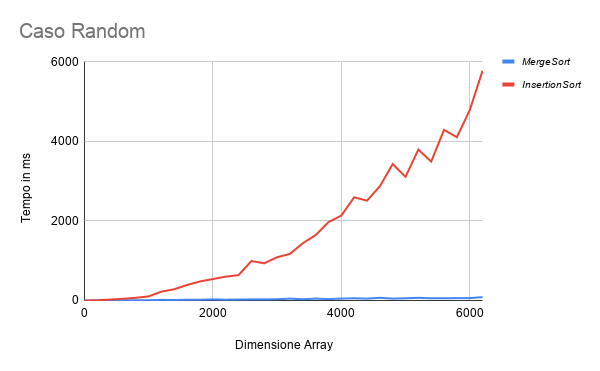
\includegraphics[width=\textwidth]{Caso Random.png}
\caption{Ordinamento di array causale}
\end{figure}
\begin{figure}[H]
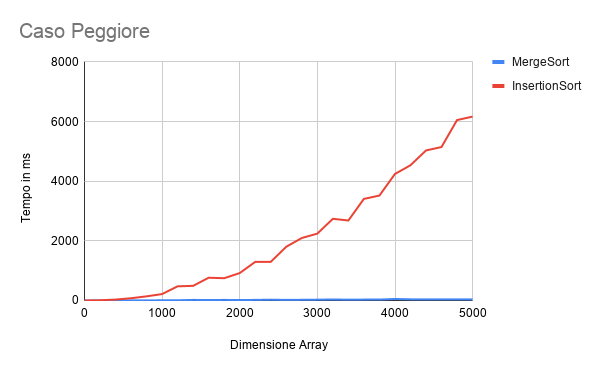
\includegraphics[width=\textwidth]{Caso Peggiore.png}
\caption{Ordinamento di array ordinato al contrario}
\end{figure}
\begin{figure}[H]
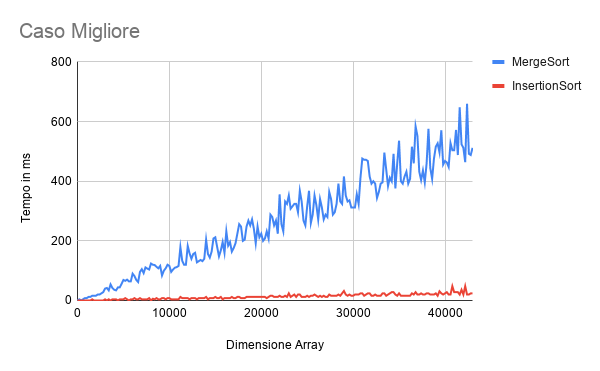
\includegraphics[width=\textwidth]{Caso Migliore.png}
\caption{Ordinamento di array ordinato}
\end{figure}
\section{Analisi risultati sperimentali}
\subsection{Analisi risultati sperimentali InsertionSort} 
Per qualsiasi dimensione degli array i risultati sono simili ed in linea con le analisi teoriche e le prestazioni attese.
\\In ogni test eseguito il tempo di esecuzione del Best-case risulta molto più veloce rispetto a qualsiasi altro tempo di esecuzione degli altri array con la stessa dimensione, infatti prendendo come esempio un array di 19800 elementi (ultimo dato riportato in tabella) si ha che il tempo di esecuzione del Best-case è circa 12ms, mentre il tempo di esecuzione di un array randomico di 6200 elementi supera i 5 secondi a seguito dei quali il programma non riesce ad elaborare l'array successivo nel tempo massimo concesso.
\\In ogni test eseguito il tempo di esecuzione del Worst-case risulta circa il doppio più lento rispetto al tempo di esecuzione degli array random della medesima dimensione. 
\\Il best-case invece risulta sempre molto più veloce anche del caso medio, infatti analizzando il grafico si vede che ha un andamento lineare rispetto al caso medio e al Worst-case. 
\\Per array di 10mila elementi il tempo di esecuzione cresce in modo drastico e c'è molta differenza tra i 3 casi. Il tempo di esecuzione del Best-case rimane molto basso invece del caso medio e del Worst-case aumenta drasticamente. Questo andamento continua anche per array crescenti.
\subsection{Analisi risultati sperimentali MergeSort}
Anche in questo caso per qualsiasi dimensione degli array i risultati sono simili ed in linea con le analisi teoriche e le prestazioni attese.
\\In ogni test con array della stessa dimensione il tempo di esecuzione degli array è molto simile tra loro. 
Nel MergeSort non esistono dei casi migliori e peggiori ma ogni array della stessa dimensione ha circa lo stesso tempo di esecuzione degli altri infatti anche quegli array che erano il Best-case e il Worst-case nell'InsertionSort, nel MergeSort hanno circa lo stesso tempo di esecuzione di un altro array generato random. 
\\Come si può vedere dal grafico, per array fino a 10mila elementi il tempo di esecuzione è compreso tra 0 e 1 secondo, si inizia a vedere un aumento del tempo di esecuzione per array di 100mila elementi che è di poco meno di 2 secondi.

\section{Conclusione}
In generale il MergeSort è un algoritmo molto più efficiente dell'InsertionSort poiché nel caso medio il MergeSort è estremamente più veloce dell'InsertionSort. Come abbiamo dimostrato praticamente nell'esercizio si ha infatti che per array molto grandi la differenza del tempo di esecuzione dei 2 algoritmi è notevole, se si deve invece ordinare array di circa 100 elementi o inferiori la differenza è appena percettibile. 
\end{document}
